\documentclass[10pt,aps,pra]{revtex4-1}

\usepackage[utf8x]{inputenc}
\usepackage[english,russian]{babel} 

\usepackage{amsmath} 
\usepackage{graphicx} 
\usepackage{verbatim} 
\usepackage{color} 
\usepackage{subfigure} 
\usepackage{hyperref} 
\usepackage{float}

\usepackage[mathlines]{lineno}


\setcounter{figure}{0}
\raggedbottom 

\begin{comment}
\pagestyle{empty} 
\end{comment}

\begin{document}

\title{Модель сложных сетей с придирчивостью}
\author{Zarvanskiy Igor, Snarskii}
\affiliation{NTUU KPI}
\affiliation{IPRI}

% \pacs{89.75.Hc }{Networks and genealogical trees}
% \pacs{02.10.Ox}{Combinatorics; graph theory}
% \pacs{89.75.-k}{Complex systems}
% \pacs{05.10.-a}{Computational methods in statistical physics and nonlinear dynamics}

\date{May 01, 2014}

\begin{abstract}
    Предлагается модификация правила предпочтительного соединения - присоединение с придирчивостью, которое применяется к моделям сетей, построенных по алгоритму Барабаши-Альберт, и для  (u,v)-flower. Приводятся результаты численного моделирования предложенных моделей и рассматриваются значения различных характеристик моделируемых сетей. Было показано, что характеристики полученных сетей ведут себя аналогично фазовым переходам второго рода, а также рассчитано пороговое значение параметра придирчивости, при котором происходит фазовый переход.
\end{abstract}

\maketitle

\linenumbers\par

\section{Введение}

    Значительное количество реальных сложных сетей являются безмасштабными сетями, такими, степени узлов которых распределяются по степенному закону. К таким сетям относятся WWW-сети, сети метаболизма, сети питания (food webs), социальные сети и многие другие \cite{Dor2}.

    В настоящее время свойства таких безмасштабных сетей подробно изучены, установлены их сетевые характеристики (средняя степень узла, минимальный средний путь, коэффициент кластеризации и т.д.) \cite{Newman1}. Необходимо заметить, что сложные сети построенные согласно \cite{AlBa2} являются идеализацией реальных сетей, характеристики которых могут иногда значительно отличаться от идеальных \cite{Newman1}. Тем не менее степенная зависимость степени узлов реальных сложных сетей встречается достаточно часто и особенно для тех сетей, которые образованы (возможно самоорганизованными) развивающимся по времени процессом \cite{Newman3, AlBa3}.

    Одним из таких процессов, который начал изучаться задолго до появления понятия сложная сеть, был процесс распределения между людьми «богатства» (под которым можно понимать деньги, вложения, недвижимость... ). Парето был установлен т.н. Закон Парето \cite{Pareto} — степенное распределение богатства – когда, число людей $\nu$, владеющих $\mu$ - долей богатства является степенной функцией $\nu \sim \mu^\gamma$, при $\gamma=0.86$ получается так, что 20\% людей владеют 80\% богатства, что часто называется законом 80/20. 

    В работе \cite{AlBa1} был найден алгоритм образования сложной сети, т.н. алгоритм Барабаши-Альберт, со степенным законом распределения степенней узлов, основанном на двух принципиально важных положениях:
        \begin{enumerate} 
            \item Сеть является растущей, начиная с некоторого затравочного числа узлов $m_0$, на каждом временном шаге появляется некоторое число новых узлов с $n$ связями.
            \item Вероятность присоединение связей от нового узла к уже существующим прямо пропорциональна степени узла.
        \end{enumerate}
    Коротко говоря модель Барабаши-Альберт — это растущая сеть с предпочтительным присоединением.

    В дальнейшем появилось много модификаций алгоритма Барабаши-Альберт, в \cite{AlBa2} их перечислено около 20-ти. Все они приводят к безмасштабным сетям с различным значением показателя степени распределения узлов по их степеням. На первый взгляд представляется, что растущая сеть с различным типом предпочтительного соединения обязательно вырастет в безмасштабную сеть.

    В настоящей работе показано, что возможна такая, незначительная на первый взгляд, модификация закона предпочтительного соединения, при которой степенное распределение модели Барабаши-Альберт нарушается. В функции распределении при этом появляется разрыв, означающий отсутствие узлов сети для некоторого диапазона значений степени. Как показали подробные исследования, введенный параметр $r$, определяющий модификацию закона предпочтительного присоединения, имеет пороговое значение $r_c$, так что при $r<r_c$ сеть остается безмаштабной сетью, а при $r \geq r_c$ появляется разрыв в функции распределения степеней узлов. Величина разрыва степенным образом зависит от близости параметра $r$ к своему пороговому значению, что позволяет говорить об аналогии с поведением параметра порядка в фазовом переходе второго рода.

    Модификация закона присоединения также была нами опробована на детерминированных иерархических безмасштабных сетях, т.н. (u,v)-flower \cite{Dor1}. При этом также наблюдалось нарушение степенной функции распределения, поведение которой аналогично поведению параметра порядка в фазовых переходах второго рода.

\section{Модель Барабаши-Альберт с придирчивостью}

    \subsection{Алгоритм Барабаши-Альберт}

        Рассмотрим растущую сеть. В стандартном варианте модели Барабаши-Альберт \cite{AlBa1} на первом шаге по времени существует $m_0$ узлов связанных между собой. На каждом следующем шаге возникает $m$ новых узлов с $q$ связями. $p_i$ - вероятность присоединения(создание связи между узлами) нового узла к уже существующему узлу $i$ пропорциональна по степени (числу связей узла $i$) - $k_i$:

            \begin{equation}
                p_i = \frac{k_i}{\sum\limits_{j} k_j},
            \end{equation}
                где суммирование происходит по всем “старым” узлам.

        Такой алгоритм, при большом числе шагов по времени приводит к степенной функции распределения степеней $P(k)$:

            \begin{equation}\label{eq:powerlaw}
                P(k) \sim k^{-\gamma},
            \end{equation}
                с показателем $\gamma =3$ \cite{AlBa1}.

        В \cite{AlBa2} приведено много модификаций правила предпочтительного присоединения, которые приводят к различным значениям показателя $\gamma$. Однак зависимость \eqref{eq:powerlaw} остается степенной.

    \subsection{Модификация алгоритма Барабаши-Альберт}

        Здесь мы предлагаем обобщение модели, основанной на правиле предпочтительного соединения, введенного Барабаши-Альберт. Новое правило предпочтительности будем для краткости называть присоединением с придирчивостью(exceptive). Согласно этой модели вводится новый параметр exceptive - $r$, принимающей значения в диапазоне $(0, 1)$. В том случае, когда выбор присоединения новой связи выпал на узел $i$ со степенью $k_i$, присоединение происходит с вероятностью $p_i$, но только в том случае, когда выполняется условие:

            \begin{equation}\label{eq:exceptive}
                p_i = \frac{k_i}{\sum\limits_{j} k_j},\quad k_i \geq r \langle k \rangle,
            \end{equation}
                где $\langle k \rangle$ – среднее значение степени узлов в сети на момент присоединение, $\langle k \rangle = \sum\limits_{j}{k_j}/{N}$.

        То есть присоединение происходит только к ``богатым'' узлам со степенью не меньше чем $r\langle k \rangle$. Введение дополнительного условия \eqref{eq:exceptive} в процессе роста сети отсекает часть узлов, то есть к ним в данный момент не может присоединиться новая связь. Необходимо заметить, что если в данный момент времени некий узел не удовлетворяет условию \eqref{eq:exceptive}, но это еще не значит, что в следующие моменты времени к нему не смогут присоединиться новые узлы, так как с течением времени изменяется значение $\langle k \rangle$.

    \subsection{Функция распределения степеней узлов}

        При значении параметра придирчивости $r=0$ предлагаемая модель переходит в стандартную модель Барабаши-Альберт, так как $k_i$ всегда больше 0. Неожиданным является наличие порогового значения параметра придирчивости $r_c$. При значении параметра придирчивости меньше некоторого порогового $r_c$, то есть при $r<r_c$ функция распределения степеней узлов $P(k)$ остается степенной, а сама сеть, тем самым, безмасштабной сетью. При значениях параметра придирчивости больше порогового значения $r \geq r_c$ сеть меняет свою структуру, а именно в сети исчезают узлы со ``средним'' количеством связей, что мы можем увидеть на рис. \ref{fig:rankDistribution_rank}. 

        Определим пороговое значение параметра придирчивости. Для этого рассчитаем сеть с начальным числом узлов $m_0 = 20$. На каждом шаге будет появляться один узел с $q=3$ связями. Делая 80 шагов строим сеть с $N=100$ узлами. Проделывая эту процедуру много раз для различных $r$ находим то значения $r$, при котором распределение $p_i$ для этой сети перестаёт быть степенным, то есть в сети появляется разрыв. Как показывают расчеты для $N=100$ $r_c(100) = 0.62$. При дальнейшем увеличении $N$ от 100 до 2000 $r_c$ уменьшается и ``насыщается'' при значении $r_c=0.51 \pm 0.04$. Это значении $r_c$ мы будем считать пороговым значением придирчивости для больших(бесконечных) сетей. Пороговое значение параметра придирчивости не изменяется при изменение начальных параметров $m_0$ и $q$. В последующих расчетах мы будем использовать $r_c=0.51 \pm 0.04$.

            \begin{figure}[H]  
                \centering
                \subfigure[]
                {
                	\label{fig:rankDistribution_rank}
                	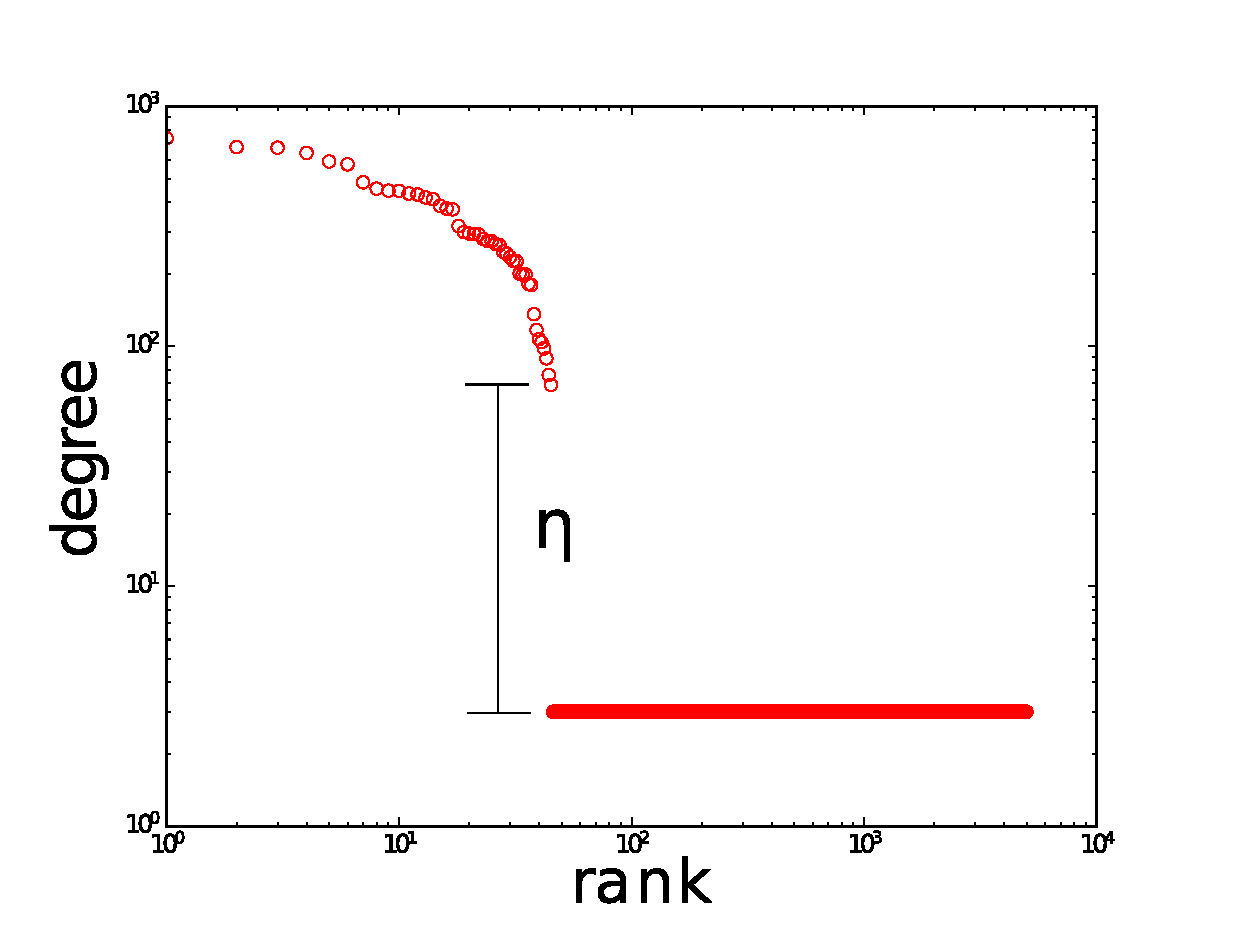
\includegraphics[height=5.5cm]{pygraph/baRank.eps}  
                }  
                \subfigure[]
                {
                	\label{fig:rankDistribution_gap}
                	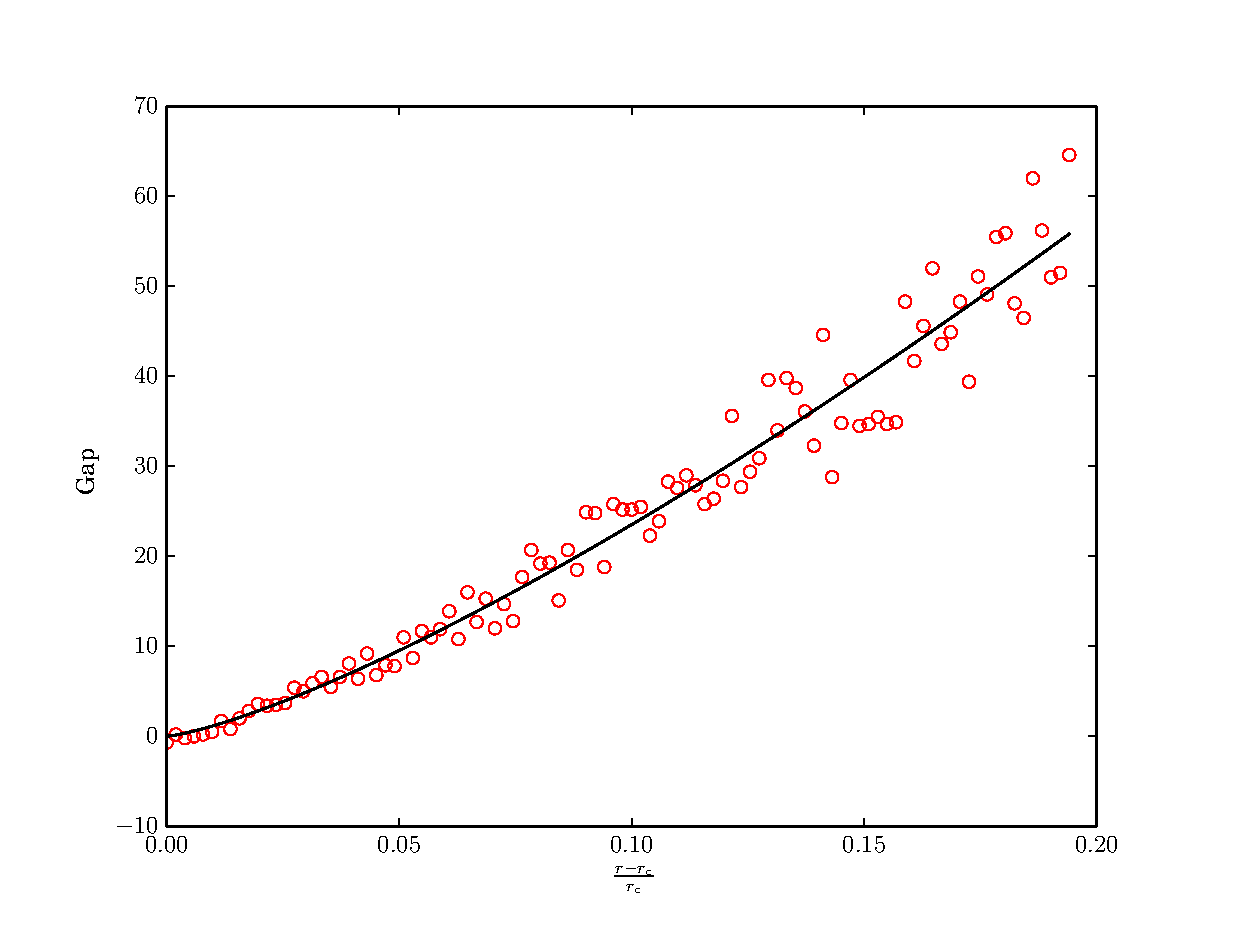
\includegraphics[height=5.5cm]{pygraph/baGap.eps} 
                }

                \caption{
                    \label{fig:rankDistribution}
                    \subref{fig:rankDistribution_rank} Оси в логарифмическом масштабе. Ранжированное распределение сети c $N=1000$ узлами при $r=0.6$. По горизонтальной оси отложено порядковый номер узла, по вертикальной оси отложена степень узла.
                    \subref{fig:rankDistribution_gap} Оси в логарифмическом масштабе. Величина разрыва при увеличении $r$ от $r_c$ до $r_c + 0.01$ с шагом $0.001$. По горизонтальной оси отложено $(r-r_c)/r_c$, по вертикальной оси отложено значение величины разрыва.
                }
            \end{figure}

        Введем новую характеристику сети - величину разрыва $\eta$ рис. \ref{fig:rankDistribution_rank}, расстояние между узлами, ближайшими к разрыву(разница значений степени узла до разрыва и после разрыва). Величина разрыва, указывает по вертикальной оси те значения степеней узлов, которые отсутствуют. 

        Поведение параметра $\eta$ аналогично поведению параметра порядка в теории фазовых переходов второго рода \cite{Landau}. Как известно, параметр порядка $\eta$, например намагниченность, при приближении температуры к критическому значению $T_c$ уменьшается степенным образом $\eta \sim (r-r_c)^\beta$, где $\beta$ – критический индекс. 

        При проведении численного эксперимента были выбраны следующие параметры: количество узлов $N=5000$, начальное количеств узлов $m_0=20$, количество связей у каждого нового узла $m=3$.

        На рис. \ref{fig:rankDistribution_gap} показана полученная зависимость $\eta = A \cdot {(r-r_c)}^\beta$, где $\beta = 1.15 \pm 0.05$.

    \subsection{Коэффициент кластеризации, коэффициент ассортативности}

        Появление разрыва $\eta$ в распределении степеней узлов $P(k)$ свидетельствует о значительном изменении структуры сети, что не может не сказаться на её характеристиках. Ниже рассмотрено поведение $C$ - коэффициента кластеризации и $A$ - коэффициента ассортативности, как функции коэффициента придирчивости $r$, при $r \geq r_c$. Для сети с $N=5000$ узлов, коэффициент кластеризации $C$, коэффициент ассортативности $A$ при $r<r_c$ от $r$ не зависит, и равны $C_0 \approx 0.01$, $A_0 \approx -0.096$, и совпадают с расчетами приведенными в \cite{AlBa2,Newman2}. 

        При увеличении $r$ от $r_c$ до $r_c + 0.01$ с шагом $0.001$ коэффициент кластеризации увеличивается от $0.04$ до $0.14$, коэффициент ассортативности уменьшается от $-0.3$ до $-0.6$(согласно рис. \ref{fig:baCharacteristic_raw}).

            \begin{figure}[H]  
                \centering
                \subfigure[]
                {
                	\label{fig:baCharacteristic_raw}
                	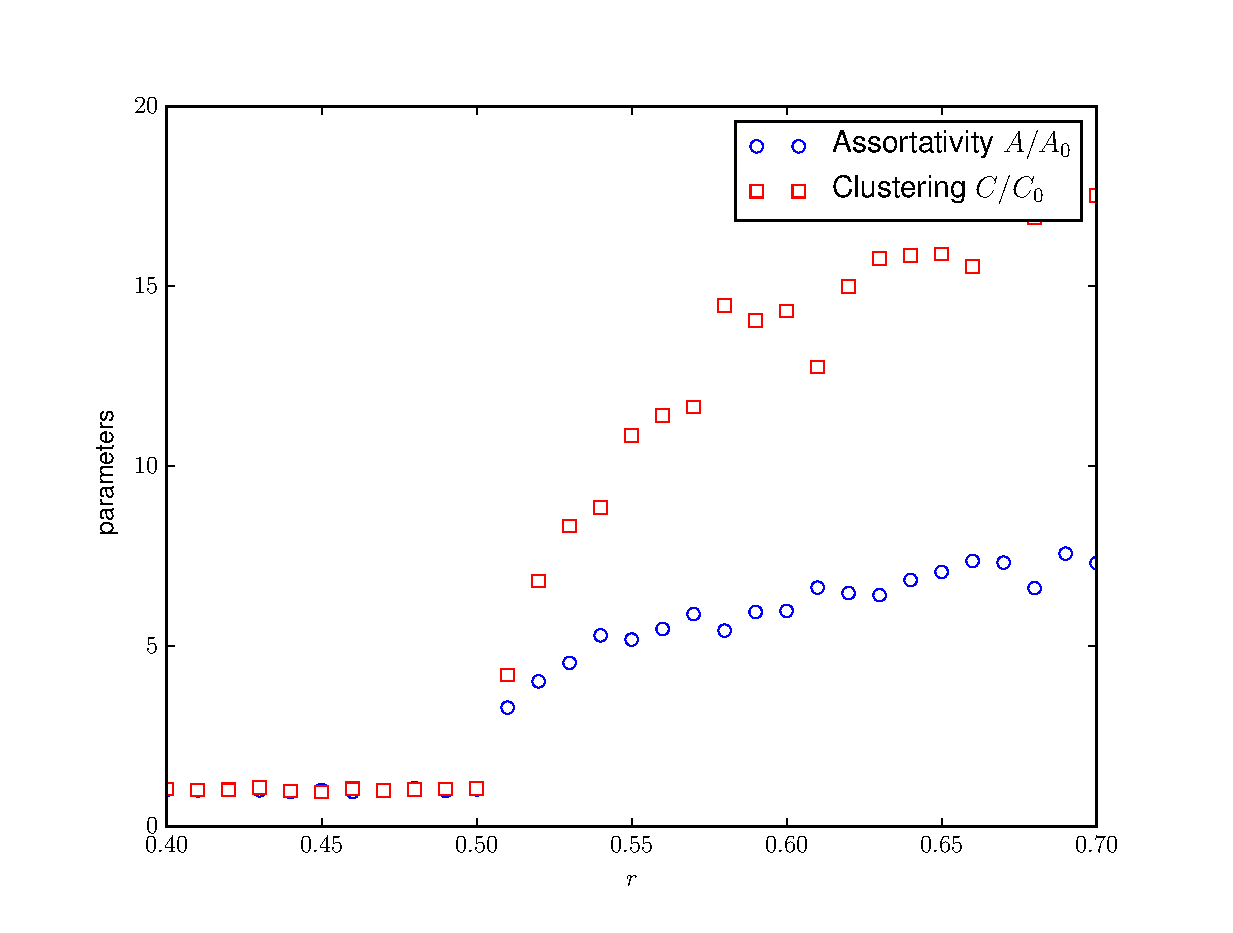
\includegraphics[height=5.5cm]{pygraph/baParams.eps}
                }  
                \subfigure[]
                {
                	\label{fig:rankDistribution_log}
                	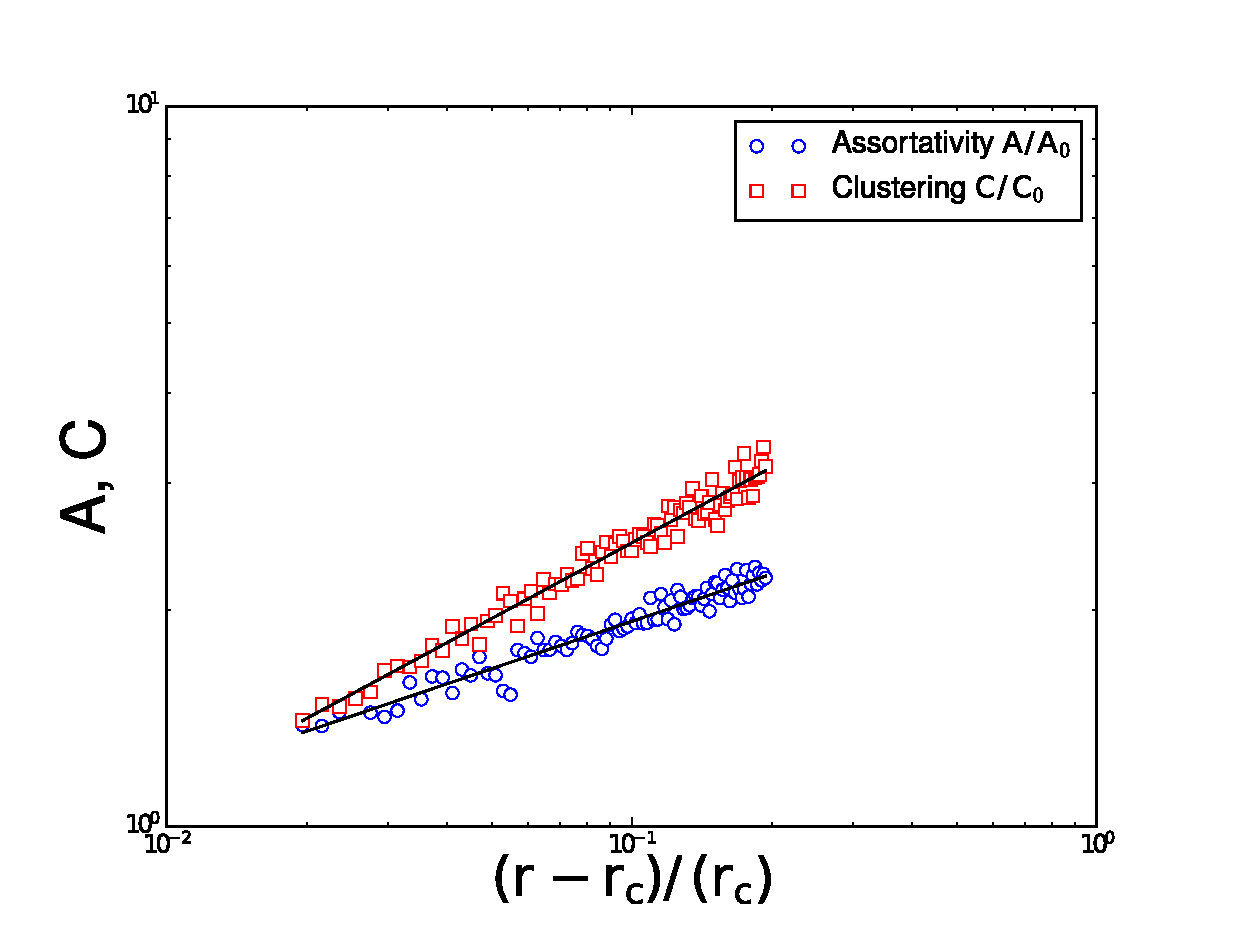
\includegraphics[height=5.5cm]{pygraph/baParamsLog.eps}
                }

                \caption{
                    \label{fig:baCharacteristic}
                    \subref{fig:baCharacteristic_raw} По горизонтальной оси отложено значение параметра придирчивости, по вертикальной оси отложено значение соответствующей характеристики. Изменение коэффициента кластеризации - C, коэффициента ассортативности - A при $r=\lceil 0,4; 0,7 \rceil$ с шагом 0.01. 
                    \subref{fig:rankDistribution_log} По горизонтальной оси отложено $(r-r_c)/r_c$, по вертикальной оси отложено значение соответствующей характеристики. Изменение коэффициента кластеризации - C, коэффициента ассортативности - A при $r=\lceil 0,5; 0,56 \rceil$ с шагом 0.0001. В двойном логарифмическом масштабе.
                }
            \end{figure}

        При $r \geq r_c$ такая зависимость появляется, и она оказывается степенной, а именно $C \sim {(r-r_c)}^\alpha$, $A \sim {(r-r_c)}^\gamma$, где $\alpha = 0.46 \pm 0.04$, $\gamma = 0.26 \pm 0.04$ (\ref{fig:rankDistribution_log}).

    \subsection{Матрица смежности для сети с придирчивостью}

        Рассмотрим матрицу смежности $A_{ij}$ для сети с придирчивостью. Для удобства нумерацию узлов в матрице смежности будем вести в порядке спадания количества связей, это означает, что $k_i=\sum\limits_{j}A_{ij}$ убывает с увеличением $i$.

            \begin{figure}[H]  
                \centering
                \subfigure[]
                {
                	\label{fig:baRankedMatrix_0}
                	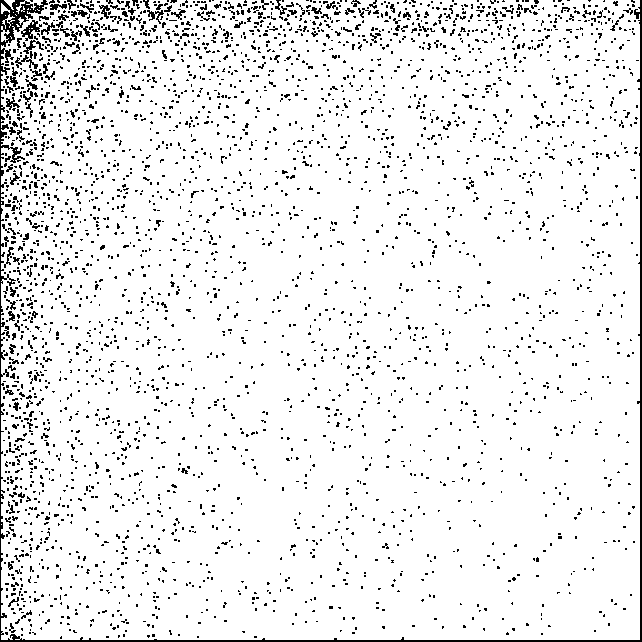
\includegraphics[height=5.5cm]{graphics/bamatrix.png}
                }  
                \subfigure[]
                {
                	\label{fig:baRankedMatrix_06}
                	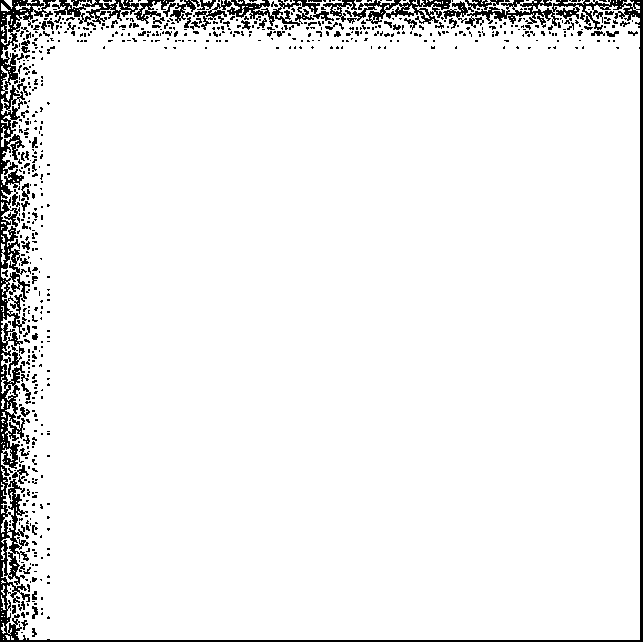
\includegraphics[height=5.5cm]{graphics/bamatrix2.png}
                }

                \caption{
                    \label{fig:baRankedMatrix}
                    Матрица смежности для сети с $N=5000$ узлов:
                    \subref{fig:baRankedMatrix_0}  при $r=0$
                    \subref{fig:baRankedMatrix_06} при $r=0.6$, где черные ячейки - это элемент с $A_ij \neq 0$.
                }
            \end{figure}

        Изменение структуры сети при $r \geq r_c$ отражается и на виде матрицы смежности. Для сети с $N=5000$ были построены две матрицы смежности: для $r<r_c$ - рис. \ref{fig:baRankedMatrix_0} и для $r>r_c$ - рис. \ref{fig:baRankedMatrix_06}. Обе матрицы были ранжированы, то есть узлы сети пронумерованы в порядке спадания количества связей $k_i$. Из рис. \ref{fig:baRankedMatrix_06} можно заметить, что в матрице смежности при $r>r_c$ в правом нижнем углу появляется значительная квадратная область, заполненная 0, то есть теми парами узлов,которые не связаны друг с другом. Эта область прямо пропорционально зависит от величины $r$.

        Таким образом такие характеристики сети, как коэффициент кластеризации и коэффициент ассортативность ведут себя аналогично параметру порядка $\eta$.

\section{Иерархические сети (u,v)-flower с придирчивостью}

    Кроме случайных безмасштабных сетей, построенных по алгоритму Барабши-Альберт(и их обобщений), известен класс простых детерминированных сетей, которые также являются безмасштабными сетями \cite{Rozenfeld2}, в частности это так называемые (u,v)-flower, рис. \ref{fig:flowerGraph}.

    Ниже мы обобщим, как и модель Барабаши-Альберт, модель (u,v)-flower, введя параметр придирчивости $r$ и случайность в закон роста сети. Как оказывается и в этом случае поведение характеристик сети аналогично поведению параметра порядка в фазовых переходах второго рода.

    \subsection{Алгоритм (u,v)-flower}

        Детерминированные растущие SF-сети, называемые (u,v)-flower и (u,v)-trees были предложены и исследованы в \cite{Dor1,Rozenfeld1,Rozenfeld2}.

            \begin{figure}[H]
                \centering
                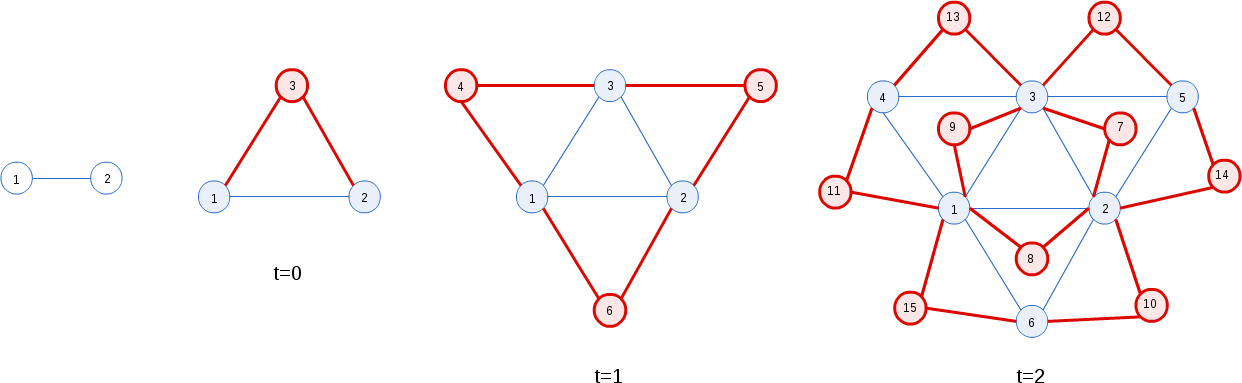
\includegraphics[height=5.5cm]{graphics/hierarhical.png}
                \caption{
                \label{fig:flowerGraph}
                    Схема построения (1,2)-flower на шагах $t=0,1,2$. Утолщенные(красные online) - узлы появившиеся на данном шаге,не утолщенные (синие online) - узлы, которые появились на предыдущих шагах.}
            \end{figure}

        Нумерация узлов вообще говоря может быть любой, однако, в рассматриваемом примере можно занумеровать узлы таким образом (рис. \ref{fig:flowerGraph}), что матрица смежности $A_{ij}$ примет наиболее простой вид. Под простым видом $A_{ij}$ мы, в данном случае, понимаем такую ее структуру, что наибольшее число наибольших квадратных областей $N \times N$ в нем остаются пустыми.

            \begin{figure}[H]  
                \centering
                \subfigure[]
                {
                	\label{fig:flowerMatrix_real}
                	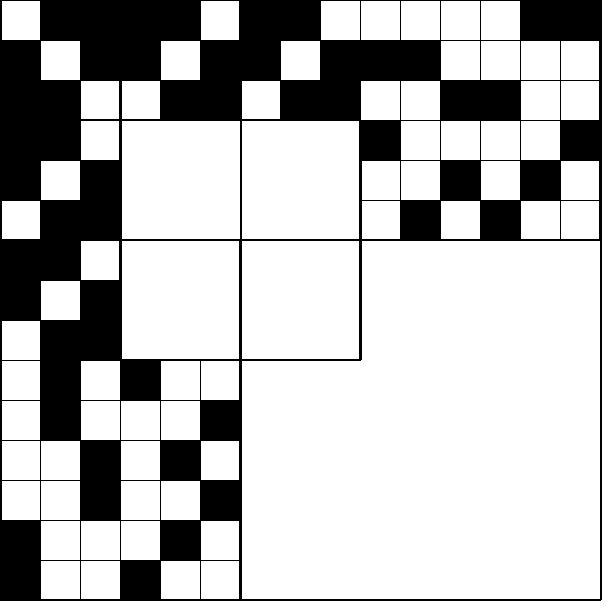
\includegraphics[height=5.5cm]{graphics/first_all_1.png}
                }  
                \subfigure[]
                {
                	\label{fig:flowerMatrix_scheme}
                	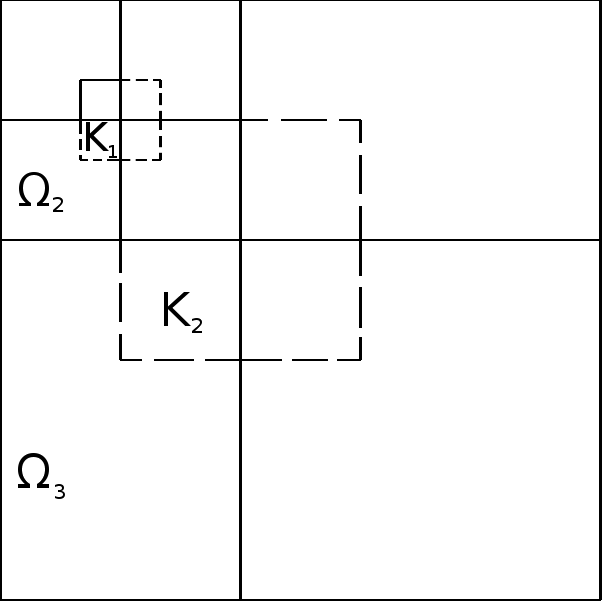
\includegraphics[height=5.5cm]{graphics/second.png}
                }

                \caption{
                    \label{fig:flowerMatrix}
                    Матрицы смежности для 3-го шага (1,2)-flower:
                    \subref{fig:baRankedMatrix_0}  матрица смежности сети с выбранной нами нумерацией
                    \subref{fig:baRankedMatrix_06} схематическое представление, где $K_1, K_2$ ... пустые
                }
            \end{figure}

        На рис. \ref{fig:flowerMatrix} - матрица смежности $N \times N$, где черные ячейки - элементы матрицы с $A_{ij}=1$. На первом шаге матрица смежности $\hat{A}$ состоит из элементов $3 \times 3$ (элементы от $A_{11} до A_{33}$, шаг $t=0$ на рис. \ref{fig:flowerGraph}). На втором шаге к ней добавляются новые элементы, и матрица состоит из $6 \times 6$ элементов(шаг $t=1$ на рис. \ref{fig:flowerGraph}). На третьем шаге шаге добавляются новые элементы, и матрица состоит из $15 \times 15$ элементов(шаг $t=2$ на рис. \ref{fig:flowerGraph}). Как видно из рис. \ref{fig:flowerMatrix} правый нижний квадрат первого шага свободен от связей и состоит из одного элемента. На втором шаге добавляется правый нижний квадрат, состоящий из $3 \times 3$ элементов, а на третьем из $9 \times 9$ элементов. На рис. \ref{fig:flowerMatrix} белым обозначены места матрицы смежности, где $A_{ij}=0$.

        При выбранной нами нумерации появляются дополнительные к построению матрицы смежности в работе \cite{Dor1} области $K_1$, $K_2$, в которых также $A_{i,j}=0$. 

        На каждом шаге $t$ имеется $N_t$ узлов и $L_t$ связей \cite{Rozenfeld1}

            \begin{equation}
                \label{eq:flowerEdgesNodesRecurent}
                N_t = (u+v) \cdot N_{t-1}-(u+v), \quad L_t=(u+v)^t.
            \end{equation}

        Т.е. на каждом шаге $t$ появляется $N_t-N_{t-1}$ узлов и $L_t-L_{t-1}$ связей. Например, рис. \ref{fig:flowerGraph}, на шаге $t=1$ появляется 3 узла и 6 связей.

        Согласно \cite{Rozenfeld1} обозначим $(u+v)=w$ и раскроем рекуррентные формулы (\ref{eq:flowerEdgesNodesRecurent}):

            \begin{equation}
                \label{eq:flowerEdgesNodesOpenRecurent}
                N_t = \frac{w-2}{w-1} \cdot w^t+\frac{w}{w-1}, \quad L_t=w^t.
            \end{equation}

        На каждом шаге $t$ есть $\Omega_t$ клеток, которые могут быть заполнены – рис. \ref{fig:flowerMatrix}. Их число равно:

            \begin{equation}
                \label{eq:flowerEmpty}
                \begin{split}
                \Omega_{t} &=(N_t-N_{t-1}) \cdot N_t-N_{t-2}^2 = \frac{w^3-w^2-1}{w^4}N_t^2 + \frac{w^3-2w^2-2w-2}{w^3}N_t-\frac{2w^2+2w+1}{w^2} = \\
                           &= \frac{w^{2t+4}-5w^{2t+3}+8w^{2t+2}-5w^{2t+1}+4w^{2t}+w^{t+5}-3w^{t+4}+4w^{t+2}-w^5}{w^{3} \cdot (w-1)^2}.
                \end{split}
            \end{equation}

        Вероятность заполнения ячейки матрицы равна:

            \begin{equation}
                W_t=\frac{L_t-L_{t-1}}{\Omega_t}=\frac{w^{t+5}-3w^{t+4}+3w^{t+3}-w^{t+2}}{w^{2t+4}-5w^{2t+3}+8w^{2t+2}-5w^{2t+1}+4w^{2t}+w^{t+5}-3w^{t+4}+4w^{t+2}-w^5}.
            \end{equation}

        Так c каждым шагом вероятность падает и матрица смежности становится все более разряженной.
        В \cite{Dor1} было показано, что (u,v)-flower являются безмасштабными сетями. Для изображенного на рис. \ref{fig:flowerGraph} (1,2)-flower распределение узлов по степеням имеет вид $P(k) \sim k^{-(1+\ln{3} / \ln{2})}$. В общем случаи для (u,v)-flower \cite{Rozenfeld1}:

            \begin{equation}
                P(k) \sim k^{-\alpha}, \quad \alpha = 1+\frac{\ln{(u+v)}}{\ln{2}}.
            \end{equation}

    \subsection{Модификация алгоритма (u,v)-flower}

        Рассмотрим случай, когда при построении (u,v)-flower не все связи реализуются. При чем вероятность отсутствия связи тем больше, чем меньше степени узлов она соединяет.

            \begin{figure}[H]
                \centering
                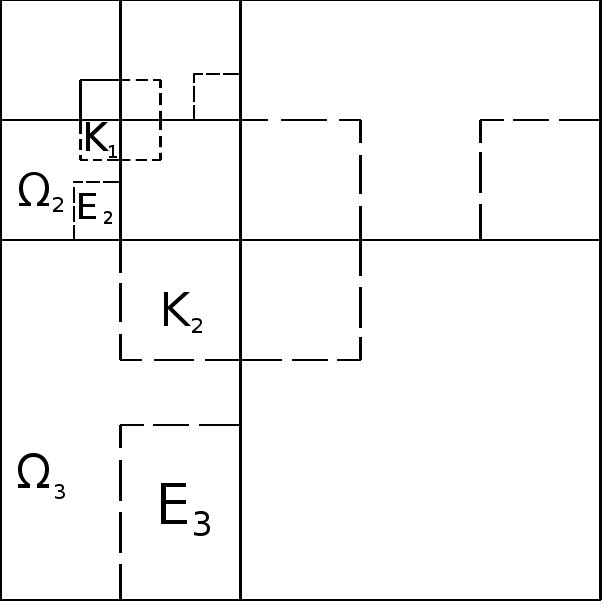
\includegraphics[height=5.5cm]{graphics/third_n.png}
                \caption{
                \label{fig:flowerMatrixExceptive}
                    Схема матрицы смежности для 3-го шага (1,2)-flower.}
            \end{figure}

        Правило присоединения с придирчивостью, как можно увидеть в случае с моделью Барабаши-Альберт \ref{fig:baRankedMatrix_06}, приводит к появлению пустой области(область без связей) в правом нижнем углу матрицы смежности. В случае с моделью (u,v)-flower такая область уже существует, поэтому мы будем делать пустые области $E_1, E_2...$  в правом нижнем углу уже заполненных областей $\Omega_1, \Omega_2...$ .

        Построение сети будем проводить путем заполнения в матрице смежности областей $\Omega_t - E_t$ с количеством связей $L_t$. Для того чтобы случайное создание связей соответствовало (u, v)-flower, необходимо сохранить закон распределению степеней узлов $p \sim k^{-(1+\ln(u+v)/\ln{2})}$\cite{Rozenfeld2}. Для сохранения закона распределения степеней узлов используется разбиение областей $\Omega_t-E_t$ на 4 равных части с вероятностью заполнения части t: $\psi_t =  \frac{1}{t}^{-(1+\ln(u+v)/\ln{2})} - \psi_{t-1}$. В последующих расчетах моделируются (1, 2)-flowers, таким образом вероятности заполнения областей $\Omega_t-E_t$ - [0.37, 0.3, 0.22, 0.11].


        Таким образом придирчивость в матрице смежности отображается правыми нижними углами областей $\Omega$ - пустыми областями $E_t$ (рис. \ref{fig:flowerMatrixExceptive}). 
        
        При моделировании использовались пустые области $E_t$ пропорциональные областям $\Omega_t$:

            \begin{equation}
                E_t= [r \cdot N_{t-1}] \cdot [r \cdot (N_t - N_{t-1})],
            \end{equation}
                где $r \cdot N_{t-1}$ - число строк, а $r \cdot (N_t - N_{t-1})$ - число столбцов областей $E_t$ в матрице смежности (рис. \ref{fig:flowerMatrixExceptive})

        Вероятность заполнения ячейки матрицы:
        
            \begin{equation}
                W_t=\psi_t \cdot \frac{L_t-L_{t-1}}{\Omega_t-E_t},
            \end{equation}
                где $\psi_t$ вероятность заполнения областей $\Omega_t - E_t$.

    \subsection{Функция распределения степеней узлов}

        При значении параметра придирчивости $r=0$ предлагаемая модель принимает вид стандартной (u,v)-flower. Как и в случае с моделью Барабаши-Альберт, в модели (u,v)-flower присутствует пороговое значения параметра придирчивости $r_c$. При значении параметра придирчивости меньше некоторого порогового $r<r_c$ функция распределения степеней узлов $P(k)$ остается степенной, а сама сеть, тем самым, безмасштабной сетью. При значениях параметра придирчивости больше порогового значения $r \geq r_c$ сеть меняет свою структуру. 

        Определим пороговое значение параметра придирчивости. Для этого рассчитаем пороговое значение для (1,2)-flower с 1 по 14 поколение. Как и в модели Барабаши-Альберт с придирчивостью происходит насыщение порогового значения. Для восьмого поколения $r_c$ полностью насыщается и мы получаем $r_c=0.75 \pm 0.04$. 

            \begin{figure}[H]  
                \centering
                \subfigure[]
                {
                	\label{fig:flowerRank_08}
                	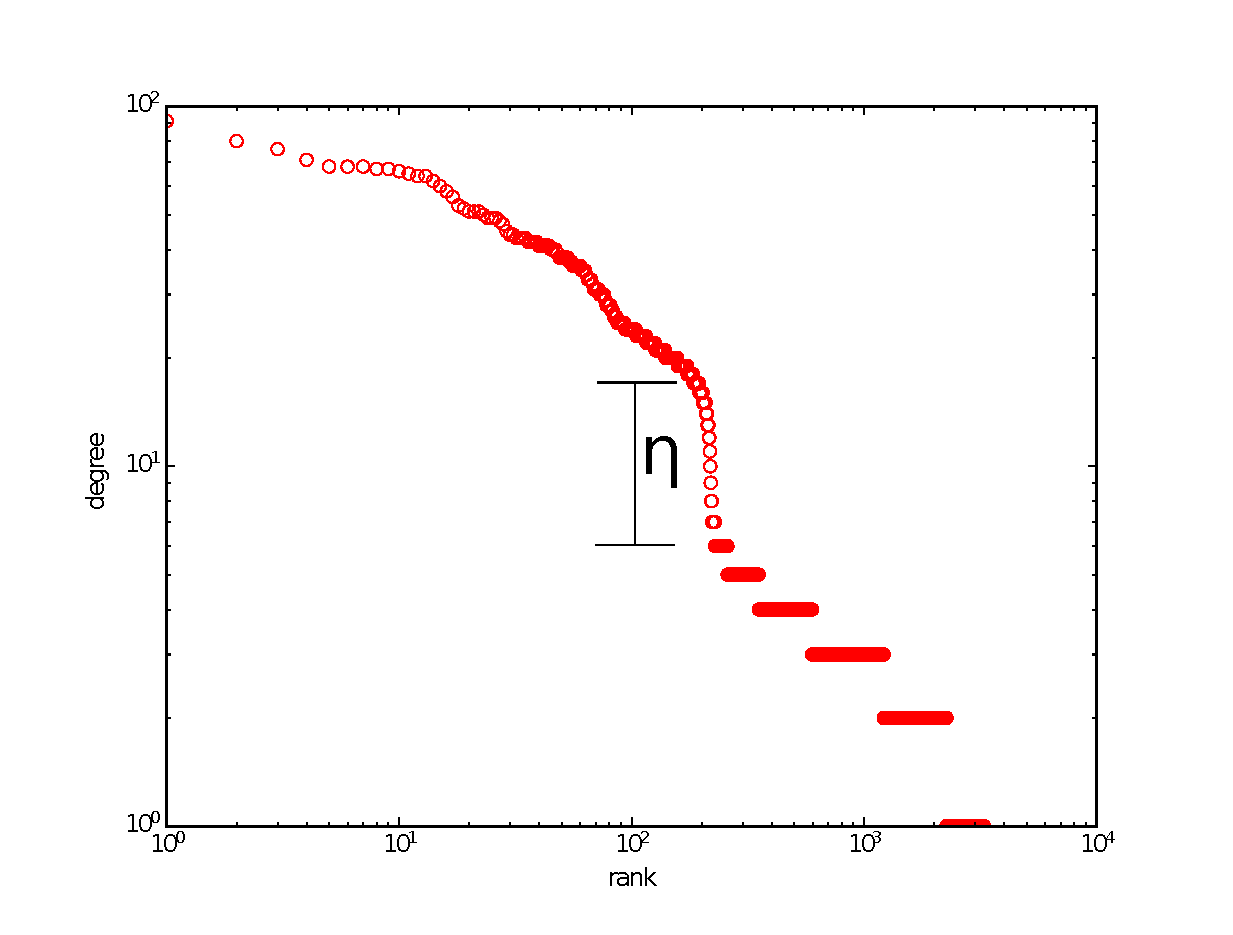
\includegraphics[height=4cm]{pygraph/flowerRank.eps}
                }
                \subfigure[]
                {
                	\label{fig:flowerRank_gap}
                	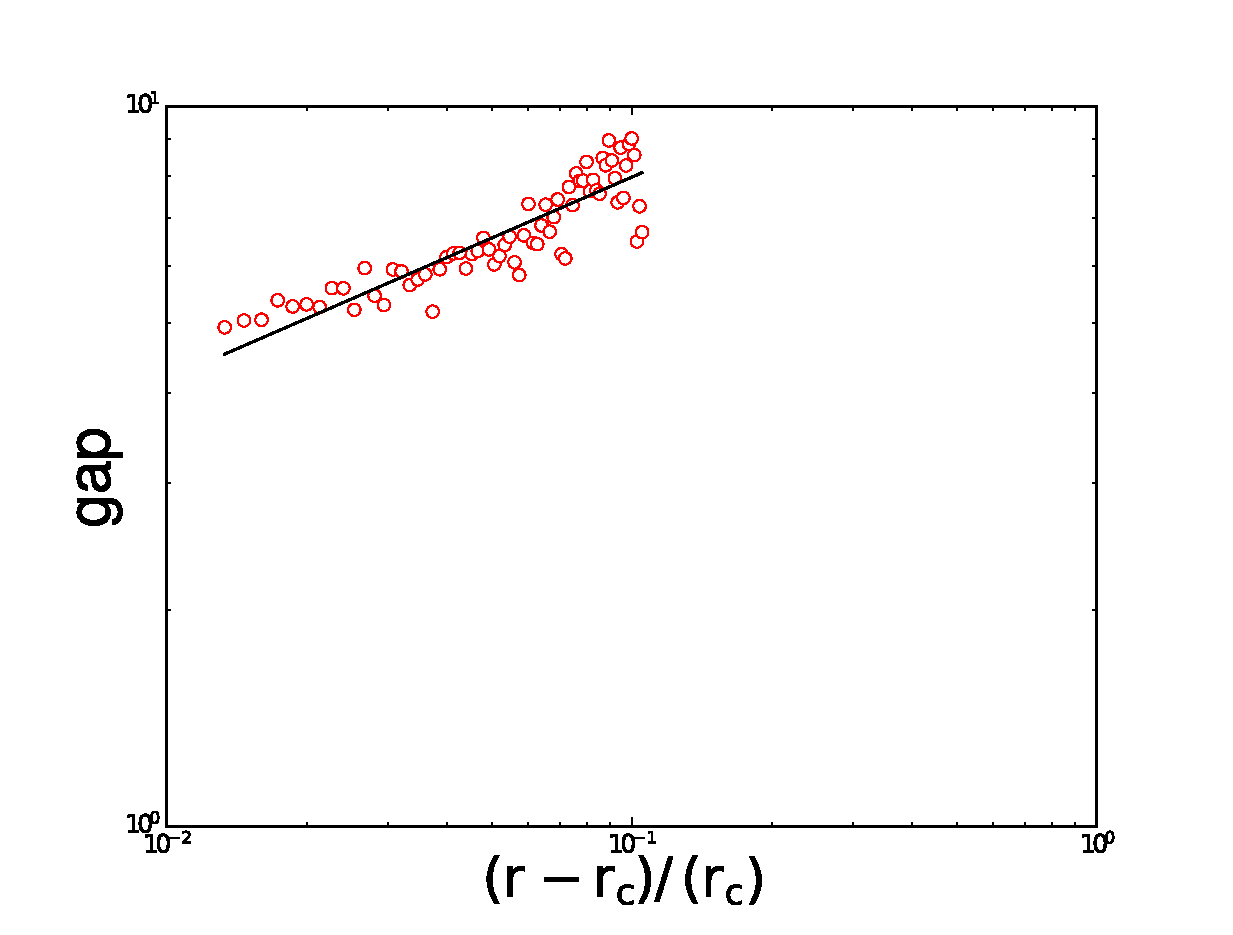
\includegraphics[height=4cm]{pygraph/flowerGap.eps}
                }

                \caption{
                    \label{fig:flowerRank}
                    \subref{fig:flowerRank_08} Оси в логарифмическом масштабе. Ранжированное распределение сети при $r=0.8$. По горизонтальной оси отложено порядковый номер узла, по вертикальной оси отложена степень узла.
                    \subref{fig:flowerRank_gap} Оси в логарифмическом масштабе. Величина разрыва при $r=\lceil 0,75; 0,83 \rceil$ с шагом 0.01. По горизонтальной оси отложено $(r-r_c)/r_c$, по вертикальной оси отложено значение величины разрыва.
                }
            \end{figure}

        Для определение значения величины разрыва (параметр $\eta$) необходимо определить точки перегиба (согласно рис. \ref{fig:flowerRank_08}). Искомые точки будут соответствовать минимумам радиуса кривизны $k=\frac{(\sqrt{1+y'^2})^3}{|y''|}$ \cite{Hazewinkel}, где $y$ аппроксимирующая функция $y=a+bx+c \cdot arctan(x) + d \cdot arctan(\alpha x + \beta)$ \cite{Mills}, $y$ - степень узла, $x$ - порядковый номер узла (согласно рис. \ref{fig:flowerRank_08}).

        Параметра $\eta$ ведет себя аналогично параметру порядка в теории фазовых переходов второго рода \cite{Landau}. Параметр $\eta$ при приближении к критическому значению уменьшается степенным образом $\eta \sim (r-r_c)^\beta$, где $\beta$ – критический индекс. 
        Моделировались сети (1,2)-flower восьмого поколения, которые содержат $N=3282$ узлов.

        На рис. \ref{fig:flowerRank_gap} показана полученная зависимость $\eta = A \cdot {(r-r_c)}^\beta$, где $\beta = 0.28 \pm 0.05$

    \subsection{Коэффициент кластеризации, коэффициент ассортативности}

        Ниже рассмотрено поведение $C$ - коэффициента кластеризации, $A$ - коэффициента ассортативности, как функции параметра придирчивости $r$, при $r \geq r_c$. Для сети (1,2)-flower восьмого поколения с $N=3282$ узлов, коэффициент кластеризации $C$, коэффициент ассортативности $A$ при $r<r_c$ от $r$ не зависит и равна $C_0 \approx 0.02$, $A_0 \approx -0.18$, что, как и должно быть, совпадает с расчетами приведенными в \cite{Rozenfeld1,Rozenfeld2}. 

        При увеличении $r$ коэффициент кластеризации увеличивается, коэффициент ассортативности уменьшается.

            \begin{figure}[H]  
                \centering
                % \subfigure[]
                % {
                % 	\label{fig:flowerParam_raw}
                % 	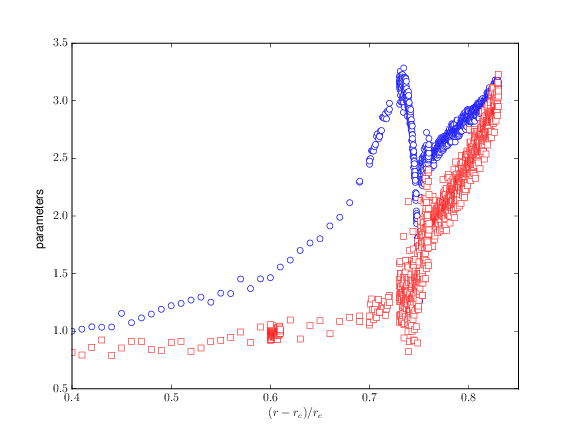
\includegraphics[height=5.5cm]{pygraph/flowerParams.png}
                % }  
                \subfigure[]
                {
                	\label{fig:flowerParam_log}
                	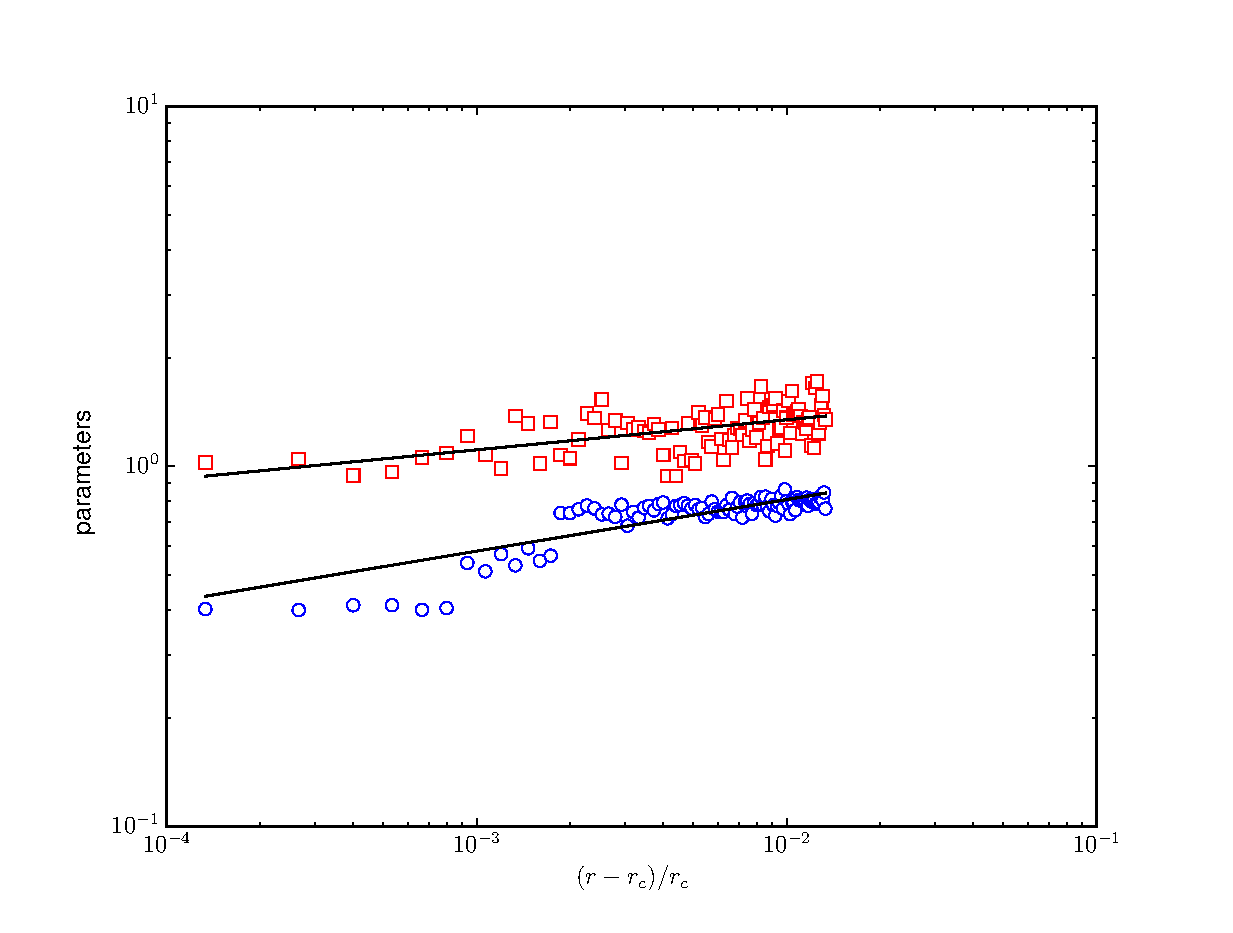
\includegraphics[height=5.5cm]{pygraph/flowerParamsLog.eps}
                }

                \caption{
                    \label{fig:flowerParam}
                    Зависимость коэффициента кластеризации и коэффициента ассортативности от $r (r>r_c)$ при $r=\lceil 0,75; 0,76 \rceil$ с шагом 0.0001.
                    % По горизонтальной оси отложено значение параметра придирчивости, по вертикальной оси отложено значение соответствующей характеристики.
                    % % \subref{fig:flowerParam_log} Изменение кластеризации, ассортативности при $r=\lceil 0,4; 0,83 \rceil$. 
                    % \subref{fig:flowerParam_log} Изменение коэффициента кластеризации, коэффициента ассортативности при $r=\lceil 0,75; 0,76 \rceil$ с шагом 0.0001. В двойном логарифмическом масштабе.
                }
            \end{figure}

        При $r \geq r_c$ такая зависимость появляется, и она оказывается степенной, а именно $C \sim {(r-r_c)}^\alpha$, $A \sim {(r-r_c)}^\gamma$, где $\alpha = 0.11 \pm 0.04$, $\gamma = 0.08 \pm 0.04$ (\ref{fig:flowerParam_log}).

\section{Заключение}

    В статье предложено модифицированное правило предпочтительного присоединения, а именно присоединение с придирчивостью, применительно к классам безмастшабных сетей - модель Барабаши-Альберт и (u,v)-flower. Модификация правила предпочтительного присоединение заключается в введении параметра придирчивости, который в процессе роста сети отсекает часть узлов,  то есть к ним в данный момент не может присоединиться новая связь

    Численное моделирование показало, что в моделируемых классах сетей происходят существенные структурные изменения. Введение новой характеристики сети - величины разрыва, и расчет уже известных характеристик, таких как коэффициент кластеризации, коэффициент ассортативности и среднее наименьшее расстояние между узлами, позволили сделать вывод о том что в моделируемых классах сетей происходит фазовый переход второго рода. Было вычислено пороговое значение при котором происходит фазовый переход, а также определено, что введенная характеристика ``величина разрыва'' пропорциональна параметру порядка.

    Появление разрыва $\eta$ при $r>r_c$ в ранжированном распределении узлов сети (\ref{fig:rankDistribution}) может представлять интерес для экономических моделей, рассматривающих распределение богатства \cite{Economics2}.

    Рассмотрим следующую модель, описывающую распределение доходов. Пусть каждый узел представляет собой предприятие. Величину богатства данного предприятия будем считать пропорциональной числу его связей с другими предприятиями, т.е. степени узла. Каждое новое предприятие (узел) соединяется (образует контакт) с другими, уже существующими узлами. Если это соединение происходит с вероятностью прямо пропорциональной величине богатства (степени узла) того предприятия, с которым происходит соединение, то распределение предприятий по величине богатства является распределением Парето \cite{Economics2, Economics1}, что наблюдается во многих реальных случаях \cite{Economics1}.

    Однако, если ввести параметр придирчивости, то вместо распределения Парето наблюдается распределение с разрывом (рис. \ref{fig:rankDistribution}). С точки зрения рассматриваемой экономической модели (степень узла - величина богатства предприятия и/или людей, его образующего) - это означает, что исчезает т.н. средний класс. На рис. \ref{fig:rankDistribution} видно, что предприятия с величиной богатства в диапазоне $\eta$ (это узлы со степенью приблизительно от 4 до 70.) практически отсутствуют. Т.е. существует только очень богатые предприятия/люди (узлы  с большой степенью) и бедные (с малой степенью). 
    
    Выражаем благодарность И.В.Безсуднову и Д.В.Ланде за многочисленные полезные обсужденя.

\section{Литература}

\bibliography{biblio} 
\bibliographystyle{ieeetr}

\end{document}